\usetikzlibrary{arrows}
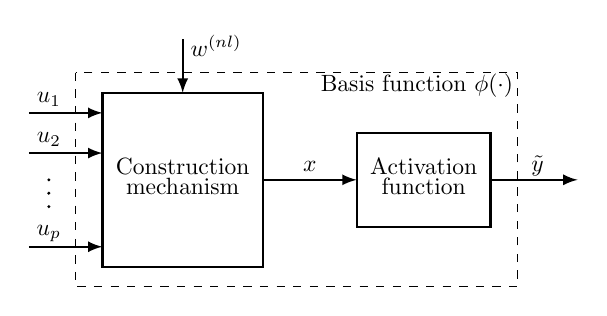
\begin{tikzpicture}[scale=0.85,transform shape]



\draw [thick] (-4.3,3.2) rectangle (-1.9,0.6);
\node at (-3.1,2.1) {Construction};
\node at (-3.1,1.8) {mechanism};
\node at (0.5,2.1) {Activation};
\node at (0.5,1.8) {function};
\draw  [thick] (-0.5,2.6) rectangle (1.5,1.2);
\draw  [thick][-latex](-1.9,1.9) -- (-0.5,1.9);
\node at (-1.2,2.1) {$x$};
\draw [thick] [-latex](1.5,1.9) -- (2.8,1.9);
\node at (2.2,2.1) {$\tilde{y}$};
\draw  [thick][-latex](-5.4,2.9) -- (-4.3,2.9);
\draw  [thick][-latex](-5.4,2.3) -- (-4.3,2.3);
\draw  [thick][-latex](-5.4,0.9) -- (-4.3,0.9);
\node at (-5.1,3.1) {$u_1$};
\node at (-5.1,2.5) {$u_2$};
\node at (-5.1,1.1) {$u_p$};

\node[circle,fill,inner sep=0.5pt] (A) at (-5.1,1.9) {};
\node[circle,fill,inner sep=0.5pt] (A) at (-5.1,1.7) {};
\node[circle,fill,inner sep=0.5pt] (A) at (-5.1,1.5) {};
\draw  [thick][-latex](-3.1,4) -- (-3.1,3.2);
\node at (-2.6,3.9) {$w^{(nl)}$};
\draw [dashed] (-4.7,3.5) rectangle (1.9,0.3);
\node at (0.4,3.3) {Basis function $\phi(\cdot)$};
\end{tikzpicture}